\documentclass[compress]{beamer}
\usepackage[brazil]{babel}
\usepackage[latin1]{inputenc}
\usepackage{amsmath}
\usepackage{graphicx}
\usepackage{listings}

%%%%%%%%%%%%%%%%%%%%%%%%%%%%%
% C O N F I G U R A � � E S %
%%%%%%%%%%%%%%%%%%%%%%%%%%%%%

\usetheme{Ilmenau}
\usecolortheme[RGB={87,130,23}]{structure}
\setbeamercovered{transparent} \setbeamertemplate{footline}[default]
\setbeamertemplate{blocks}[rounded][shadow=false]
\setlength{\tabcolsep}{1mm} \setbeamertemplate{footline}[frame
number] \setbeamertemplate{navigation symbols}{}
\renewcommand{\baselinestretch}{1}

%%%%%%%%%%%%%%%%%%%%%%%%%%%%%%%%%%%%%%%%%%%%%%%%%%%%
% C O N F I G U R A � � E S  D O S   C � D I G O S %
%%%%%%%%%%%%%%%%%%%%%%%%%%%%%%%%%%%%%%%%%%%%%%%%%%%%

\lstset{numbers=left, stepnumber=1, firstnumber=1,
numberstyle=\scriptsize, extendedchars=true,
breaklines=true,frame=tb, basicstyle=\scriptsize,
stringstyle=\scriptsize, showstringspaces=false}

\renewcommand{\lstlistingname}{C�digo}
\renewcommand{\lstlistlistingname}{Lista de C�digos}


%%%%%%%%%%%
% C A P A %
%%%%%%%%%%%

\title{Curso C\# Conceitos B�sicos}

\author{Diogo Cezar Teixeira Batista \\
       {\footnotesize\ttfamily diogocezar@utfpr.edu.br}
}

\institute{\large Universidade Tecnol�gica Federal do Paran� \\
                  Campus Corn�lio Proc�pio \\
                  UTFPR-CP}

\date{Corn�lio Proc�pio - 2008}

\begin{document}

\begin{frame}
    \titlepage
\end{frame}

\begin{frame}[t,allowframebreaks]
    \frametitle{Agenda}
    \tableofcontents
\end{frame}

%\section[Introdu��o]{Introdu��o}
\begin{frame}
    \frametitle{Introdu��o}
    \begin{itemize}

        \item <1-> Onde est� a p�gina que procuro em um site?

%        \item <1-> Grande n�mero de sistemas hiperm�dia;
%
%        \item <2-> Informa��es distribu�das desorganizadamente na Internet;
%
%        \item <3-> Sistemas de busca;
%
%            \begin{itemize}
%                \item <4-> Trazem conte�do n�o relacionado, ou
%                irrelevante (sem�ntica);
%                \item <5-> N�o oferecem assist�ncia navegacional;
%            \end{itemize}

        \item <2-> \emph{Hiperm�dia Adaptativa}: modifica��o do conte�do
        \emph{web}.

        \item <3-> Proposta: navega��o colaborativa;

            \begin{itemize}
                \item <4-> Ajuda m�tua entre os usu�rios que
                estiverem navegando pelas mesmas p�ginas;

                \item <5-> Solu��o baseada na teoria do comportamento das
                formigas;
            \end{itemize}

    \end{itemize}
\end{frame}

%\section[A linguagem C\#]{A linguagem C\#}
\begin{frame}
    \frametitle{A linguagem C\#}
    \begin{itemize}
        \item <1-> � uma linguagem da plataforma .NET;
        \item <2-> Derivada do C++;
        \item <3-> Orientada a objetos.
    \end{itemize}
\end{frame}

\subsection{Caracter�sticas do C\#}

\begin{frame}
    \frametitle{Caracter�sticas do C\#}
    \begin{itemize}
        \item <1-> Simplicidade;
        \item <2-> Completamente orientada a objetos;
        \item <3-> Fortemente tipada;
        \item <4-> Tudo � um objeto;
        \item <5-> Controle de vers�es;
        \item <6-> Entre outros.
    \end{itemize}
\end{frame}

\begin{frame}
    \frametitle{Caracter�sticas do C\#}
    Alguns detalhes que devem ser observados:
    \begin{itemize}
        \item <1-> Sensitive CASE, diferencia mai�sculas e min�sculas;
        \item <2-> As instru��es terminam com ponto e virgula;
        \item <3-> As extens�es dos arquivos s�o .cs;
    \end{itemize}
    \begin{block}<4->{Coment�rios}
        \small
        \textcolor[rgb]{0.00,0.50,0.00}{
        // Comenta apenas uma linha por vez \\
        \vspace{0.5cm}
        /* Este � um coment�rio de m�ltiplas linhas. \\
        Ele pode ser dividido Em muitas linhas */}
    \end{block}
\end{frame}

\subsection{Primeiro programa em C\#}

\begin{frame}
    \frametitle{Primeiro programa em C\#}
    Escrevendo o tradicional programa Hello World, em C\#:
    \texttt{\lstinputlisting[language=C, label=helloword, caption={Hello
    World em C\#}]{cods/helloworld.txt}}
\end{frame}

\begin{frame}
    \frametitle{Estrutura de um programa em C\#}
    \texttt{\lstinputlisting[language=C, label=programstructure,
    caption={Estrutura de um programa em
    C\#}]{cods/programstructure.txt}}
\end{frame}

\begin{frame}
    \frametitle{Estrutura de um programa em C\#}
    \begin{itemize}
        \item <1-> \emph{Namespaces}: s�o a forma l�gica de organizar o c�digo-fonte;
        \item <2-> Tipos: classes, estruturas, interfaces, delega��es, enums;
        \item <3-> Membros: constantes, campos, m�todos, propriedades, indexadores, eventos, operadores, construtores;
        \item <4-> Outros: com�ntarios e instru��es.
    \end{itemize}
\end{frame}

\subsection{Tipos de dados em C\#}

\begin{frame}%[t,allowframebreaks]
    \frametitle{Tipos de dados em C\#}
        \tiny
        \vspace{-1cm}
        \begin{table}[!htb]
            \centering
            \label{tab:tiposprimitivos}
            \caption{Tipos primitivos do C\#}
            \begin{tabular}{|l|l|p{4cm}|p{3.5cm}|}
                \hline
                Tipo C\# & Tipo .NET & Descri��o & Faixa de dados \\
                \hline
                bool & System.Boolean & Booleano & true ou false \\
                \hline
                byte & System.Byte & Inteiro de 8-bit com sinal & -127 a 128 \\
                \hline
                char & System.Char & Caracter Unicode de 16-bit & U+0000 a U+ffff \\
                \hline
                decimal & System.Decimal & Inteiro de 96-bit com sinal com 28-29 d�gitos significativos & 1,0 x $10^{-28}$ a 7,9 x $10^{28}$ \\
                \hline
                double & System.Double & Flutuante IEEE 64-bit com  & +-5,0 x $10^{-324}$ a +-1,7 x $10^{324}$ \\
                \hline
                float & System.Single & Flutuante IEEE 32-bit com  & +-1,5 x $10^{-45}$ a +-3,4 x $10^{38}$ \\
                \hline
                int & System.Int32 & Inteiro de 32-bit com sinal & -2.147.483.648 a 2.147.483.647 \\
                \hline
                long & System.Int64 & Inteiro de 64-bit com sinal & -9,223,372,036,854,775,808 a 9,223,372,036,854,775,807 \\
                \hline
                Object & System.Object & Classe base  &  -\\
                \hline
                Sbyte & System.Sbyte & Inteiro de 8-bit sem sinal & 0 a 255 \\
                \hline
                Short & System.Int16 & Inteiro de 16-bit com sinal & -32,768 a 32,767 \\
                \hline
                String & System.String & String de caracteres Unicode &  -\\
                \hline
                Uint & System.UInt32 & Inteiro de 32-bit sem sinal & 0 a 4,294,967,295 \\
                \hline
                Ulong & System.UInt64 & Inteiro de 64-bit sem sinal & 0 a 18,446,744,073,709,551,615 \\
                \hline
                Ushort & System.UInt16 & Inteiro de 16-bit sem sinal & 0 a 65,535 \\
                \hline
            \end{tabular}
        \end{table}
\end{frame}

\begin{frame}
    \frametitle{Tipos Valor e Tipos Refer�ncia}
    \begin{itemize}
            \item <1-> Tipos valor(\emph{value types}): dados em mem�ria;
            \item <2-> Tipos refer�ncia(\emph{reference types}): refer�ncia para um valor;
            \item <3-> Tipos ponteiro(\emph{pointer types}): apontam para um endere�o de mem�ria.
        \end{itemize}
\end{frame}

\begin{frame}
    \frametitle{Convers�o de tipos}
    \begin{itemize}
            \item <1-> Valores s�o convertidos sempre para o tipo de maior faixa de valores;
            \item <2-> A convers�o dos tipos de ponto flutuante(float, double) para decimal causa erro;
            \item <3-> A convers�o entre os tipos com sinal e sem sinal de valores inteiros com o mesmo tamanho causa erro.
    \end{itemize}
\end{frame}

\begin{frame}
    \frametitle{Tipos de convers�o autom�tica}
       \scriptsize
        \vspace{-1cm}
        \begin{table}[!htb]
            \centering
            \label{tab:conversaoautomatica}
            \caption{Tipos de convers�o autom�tica}
            \begin{tabular}{|l|l|}
                \hline
                Tipo & Converte em \\
                \hline
                sbyte & short, int, long, float, double, decimal \\
                \hline
                byte & short, ushort, int, uint, long, ulong, float, double, decimal \\
                \hline
                short & int, long, float, double, decimal \\
                \hline
                ushort & int, uint, long, ulong, float, double, decimal \\
                \hline
                int & long, float, double, decimal \\
                \hline
                uint & long, ulong, float, double, decimal \\
                \hline
                long & float, double, decimal \\
                \hline
                ulong & long, double, decimal \\
                \hline
                char & ushort, int, uint, long, ulong, float, double, decimal \\
                \hline
                float & double \\
                \hline
            \end{tabular}
        \end{table}
\end{frame}

\begin{frame}
    \frametitle{O Objeto \emph{Convert}}
    \begin{itemize}
            \item Em C\# temos o objeto \texttt{\emph{Convert}} que � usado para converter um tipo de dado em
            outro;
            \item  Os tipos de dados suportados s�o: \emph{Boolean}, \emph{Char},
            \emph{SByte}, \emph{Byte}, \emph{Int16}, \emph{Int32}, \emph{Int64},
            \emph{UInt16}, \emph{UInt32}, \emph{UInt64}, \emph{Single},
            \emph{Double}, \emph{Decimal}, \emph{DateTime} e \emph{String}.
    \end{itemize}

    \texttt{\lstinputlisting[language=C, label=conversaoConvert,
    caption={Exemplo de utiliza��o do objeto Convert}]{cods/conversaoconvert.txt}}
\end{frame}

\subsubsection{Arrays}

\begin{frame}[t,allowframebreaks]
    \frametitle{Arrays}
    \begin{itemize}
            \item \emph{array} � uma matriz de valores do mesmo tipo, criada em tempo de execu��o, acessada por meio de um �ndice;
            \item declara��o do \emph{array} sempre faz o uso de um colchete([]);
            \item O tipo \emph{array} pode ter diversas dimens�es;
    \end{itemize}
    \texttt{\lstinputlisting[language=C, label=array, caption={Sintaxe
    para a declara��o de Arrays}]{cods/array.txt}}

    \texttt{\lstinputlisting[language=C, label=array2, caption={Sintaxe
    para a declara��o de Arrays com duas ou mais
    dimens�es}]{cods/array2.txt}}

    \texttt{\lstinputlisting[language=C, label=array3, caption={Sintaxe
    para a declara��o de uma matriz de Arrays com duas ou mais
    dimens�es}]{cods/array3.txt}}

    \texttt{\lstinputlisting[language=C, label=array4, caption={Sintaxe
    para a inicializa��o de Arrays com duas ou mais
    dimens�es}]{cods/array4.txt}}

    \begin{itemize}
            \item Para passar um argumento array para um m�todo, especifique o nome do array sem usar colchetes.
            \item Para que um m�todo receba um \emph{array}, a lista de par�metros deve especificar que um array ser� recebido.
    \end{itemize}

    \texttt{\lstinputlisting[language=C, label=array5, caption={Passando arrays � m�todos}]{cods/array5.txt}}

    \begin{block}{Propriedades e M�todos dos Arrays}
        \begin{itemize}
            \item \texttt{obj.Length} $\longrightarrow$ Tamanho do vetor;
            \item \texttt{Array.IndexOf(Array vetor, object value)} $\longrightarrow$ Procura a primeira ocorr�ncia de valor em vetor;
            \item \texttt{Array.LastIndexOf(Array vetor, object value)} $\longrightarrow$ Procura a �ltima ocorr�ncia de valor em vetor;
            \item \texttt{Array.Sort(Array vetor)} $\longrightarrow$ Ordena um vetor crescentemente;
            \item \texttt{Array.Reverse(Array vetor)} $\longrightarrow$ Ordena um vetor decrescentemente.
        \end{itemize}
    \end{block}
\end{frame}

%\section{Comandos}

\subsection{Sele��o}

\begin{frame}
    \frametitle{Comandos de Sele��o}
    \begin{itemize}
            \item <1-> Escolha de uma possibilidade entre uma ou mais poss�veis;
            \item <2-> Os comandos \texttt{\emph{if}} e \texttt{\emph{switch}} fazem parte deste grupo.
    \end{itemize}
\end{frame}

\subsubsection{Comando If}

\begin{frame}
    \frametitle{Comando de Sele��o If}
    \begin{itemize}
            \item Express�o booleana para executar um bloco de comando;
            \item Cl�usula else opcional.
    \end{itemize}
    \texttt{\lstinputlisting[language=C, label=if, caption={Exemplo do
    comando If em C\#}]{cods/if.txt}}
\end{frame}

\begin{frame}
    \frametitle{Operador tern�rio}
    \begin{itemize}
            \item \emph{If} com a cl�usula \emph{else} �nica;
            \item Tern�rio: 3 express�es;
            \item Representado por interroga��o;
    \end{itemize}
    \texttt{\lstinputlisting[language=C, label=if6, caption={Operador
    Tern�rio}]{cods/if6.txt}}
\end{frame}

\subsubsection{Comando Switch}

\begin{frame}
    \frametitle{Comando de Sele��o Switch}
    \begin{itemize}
            \item Switch: interruptor;
            \item Verifica se um valor existe em uma lista de op��es;
    \end{itemize}
    \texttt{\lstinputlisting[language=C, label=switch, caption={Comando
    Switch}]{cods/switch.txt}}
\end{frame}

\begin{frame}
    \frametitle{Break e Continue}
    \begin{itemize}
            \item <1-> \emph{Break}: Utilizada para sa�da prematuramente de um la�o ou uma instru��o \emph{switch};
            \item <2-> \emph{Continue}: Pula as instru��es restantes no corpo da estrutura e passa para a pr�xima itera��o do la�o;
    \end{itemize}
\end{frame}

\subsection{Itera��o ou Loop}

\begin{frame}
    \frametitle{Comandos de Itera��o ou Loop}
    \begin{itemize}
            \item Conhecidos como la�o ou loop;
            \item Executam repetidamente um comando ou bloco de comandos;
            \item Encerram o ciclo com uma condi��o;
    \end{itemize}
\end{frame}

\subsubsection{Comando For}

\begin{frame}
    \frametitle{Comando de Itera��o For}
    \begin{itemize}
            \item Possui 3 declara��es opcionais;
            \item Separadas por ponto e v�rgula (;);
            \item Declara��es: inicializa��o, condi��o e itera��o;
            \item Mais de uma express�o em cada par�metro: separa��o por v�rgula(,).
    \end{itemize}
    \texttt{\lstinputlisting[language=C, label=for, caption={Itera��o
    For}]{cods/for.txt}}
\end{frame}

\subsubsection{Comando Foreach}

\begin{frame}
    \frametitle{Comando de Itera��o Foreach}
    \begin{itemize}
            \item Enumera os elementos de uma cole��o;
    \end{itemize}
    \texttt{\lstinputlisting[language=C, label=foreach,
    caption={Itera��o foreach (exemplo)}]{cods/foreach.txt}}
\end{frame}

\subsubsection{Comandos do e while}

\begin{frame}
    \frametitle{Comandos de Itera��o do e while}
    \begin{itemize}
            \item Caracter�sticas semelhantes;
            \item Executam condicionalmente um comando ou bloco de comandos;
            \item Comando \emph{do} $\longrightarrow$ executado uma ou mais vezes;
            \item Comando \emph{while} $\longrightarrow$ executado nenhuma ou mais vezes;
    \end{itemize}
    \texttt{\lstinputlisting[language=C, label=dowhile,
    caption={Itera��o do while (exemplo)}]{cods/dowhile.txt}}
\end{frame}

%\section{Operadores}

\begin{frame}
    \frametitle{Operadores em C\#}
    \begin{itemize}
            \item <1-> C\# � uma linguagem muito rica em operadores;
            \item <2-> Representados por s�mbolos;
            \item <3-> Utilizados na constru��o de express�es;
            \item <4-> Sintaxe � baseada na sintaxe do C++;
            \item <5-> M�ltiplas opera��es: preced�ncia dos operadores (pode ser modificado por par�nteses);
    \end{itemize}
\end{frame}

\begin{frame}%[t,allowframebreaks]
    \frametitle{Operadores do C\#}
        \tiny
        \vspace{-1cm}
        \begin{table}[!htb]
            \centering
            \label{tab:tiposprimitivos}
            \caption{Operadores do C\#}
            \begin{tabular}{|l|l|}
                \hline
                Categoria & Operadores \\
                \hline
                Aritm�tica &\& + - * / \% \\
                \hline
                L�gica (boolena e bitwise) & \& $|$ \^{} ! ~ \&\& $||$ true false \\
                \hline
                Concatena��o de string & + \\
                \hline
                Incremento e decremento & ++ -- \\
                \hline
                Shift & $<<$ $>>$ \\
                \hline
                Relacional & == != $<>$ $<$= $>$= \\
                \hline
                Atribui��o & = += -= *= /= \%= \&= |= \^= $<<$= $>>$= \\
                \hline
                Acesso a membro & . \\
                \hline
                Indexa��o & [] \\
                \hline
                Indexa��o & () \\
                \hline
                Condicional & ?: \\
                \hline
                Delegate (concatena��o e remo��o) & + - \\
                \hline
                Delegate (concatena��o e remo��o) & new \\
                \hline
                Informa��o de tipo & is sizeof typeof \\
                \hline
                Controle de excess�o de overflow & checked unchecked \\
                \hline
                Indire��o e endere�o & * -> [] \& \\
                \hline
            \end{tabular}
        \end{table}
\end{frame}

\subsection{Operadores Aritm�ticos}

\begin{frame}
    \frametitle{Operadores Aritm�ticos}
    \begin{itemize}
            \item <1-> Usados para execu��o de c�lculos;
            \item <2-> Divididos em operadores un�rios e bin�rios;
    \end{itemize}
\end{frame}

\begin{frame}
    \frametitle{Operadores Aritm�ticos Un�rios}
    \begin{block}{Operadores Un�rios}
        (atribu�dos a 1 atributo) + e - s�o utilizados
        para representar se o n�mero � positivo ou negativo,
        respectivamente.
    \end{block}
    \texttt{\lstinputlisting[language=C, label=operadoresUnarios,
    caption={Operadores Un�rios}]{cods/operadores.txt}}
\end{frame}

\begin{frame}
    \frametitle{Operadores Aritm�ticos Bin�rios}
    \begin{block}{Operadores Bin�rios}
        +, -, *, / e  \% s�o utilizados nas
        express�es para execu��o de c�lculos tais como soma, subtra��o,
        multiplica��o, divis�o e sobra.
    \end{block}
    \texttt{\lstinputlisting[language=C, label=operadoresBinarios,
    caption={Operadores Bin�rios}]{cods/operadores2.txt}}
\end{frame}

\subsection{Operadores de Incremento e Decremento}

\begin{frame}
    \frametitle{Operadores de Incremento e Decremento}
    \begin{block}{Incremento e Decremento}
        Os operadores ++ e -- aumentam ou diminuem por um o valor
        correspondente.
    \end{block}
    \texttt{\lstinputlisting[language=C, label=operadoresIncDec,
    caption={Operadores de Incremento e
    Decremento}]{cods/operadores4.txt}}
\end{frame}

\subsection{Operadores L�gico, Relacional e Condicional}

\begin{frame}
    \frametitle{Operadores L�gico, Relacional e Condicional}
    \begin{itemize}
            \item <1-> Utilizados em express�es onde o resultado retornado ou a caracter�stica � booleana.
            \item <2-> O operador de nega��o ! retorna o complemento (contr�rio) de um valor booleano.
    \end{itemize}
    \begin{block}{Operadores L�gico, Relacional e Condicional}
        Os operadores relacionais ==, !=, $<$, $>$, $<$=, $>$=, resultam em um valor
        booleano e representam igual, n�o igual ou diferente, menor, maior,
        menor ou igual e maior ou igual, respectivamente.
    \end{block}
\end{frame}

\subsection{Opera��o de Atribui��o}

\begin{frame}
    \frametitle{Opera��o de Atribui��o}
    \begin{itemize}
            \item <1-> Divididos entre simples e compostos;
            \item <2-> Utilizados na designa��o de um valor para uma vari�vel;
            \item <3-> O operador = representa a atribui��o simples;
    \end{itemize}
    \begin{block}{Operadores de atribui��o compostos}
        Os operadores +=, -=, *=, /=, \%=, \&=, |=, \^=, $<<$= e $>>$=
        representam a atribui��o composta, que normalmente atuam como um
        atalho na constru��o de uma express�o.
    \end{block}
\end{frame}

\begin{frame}
    \frametitle{Opera��o de Atribui��o}
    \texttt{\lstinputlisting[language=C, label=operadoresAtr,
    caption={Exemplo do operador de atribui��o}]{cods/operadores6.txt}}

    \texttt{\lstinputlisting[language=C, label=operadoresAtrComp,
    caption={Exemplo do operador de atribui��o
    composta}]{cods/operadores7.txt}}
\end{frame}

%\section{Programa��o Baseada em Objetos}

\subsection{Conven��es e Padr�es de Nomenclatura}

\begin{frame}
    \frametitle{Recomenda��o da Microsoft para nomea��o de vari�veis}
    \begin{itemize}
            \item <1-> Evite usar underline "\_";
            \item <2-> N�o crie vari�veis com o mesmo nome mudando somente entre mai�sculas e min�sculas;
            \item <3-> Utilize nomes de vari�veis com min�sculas;
            \item <4-> Evite utilizar todas as letras mai�sculas;
            \item <5-> Nota��o \emph{camelCasing}: Primeira letra de cada palavra em caixa alta, menos da primeira;
            \item <6-> Recomenda��es para nomea��o de classes, m�todos: Nota��o \emph{PascalCasing}: primeiro caractere de cada palavra em
            caixa alta.
    \end{itemize}
\end{frame}

\subsection{Classes}

\begin{frame}
    \frametitle{Classes}
    \begin{block}{Defini��o}
        Uma classe � um poderoso tipo de dado em C\#. Como estrutura, uma
        classe define os dados e o comportamento dos tipos de dados.
    \end{block}
    \texttt{\lstinputlisting[language=C, label=classe, caption={Exemplo
    de Classe em C\#}]{cods/classe.txt}}
\end{frame}

\subsection{Propriedades}

\begin{frame}
    \frametitle{Propriedades}
    \begin{block}{Defini��o}
        As propriedades s�o recursos fornecidos pelas classes para que seja
        poss�vel alterar seus valores.
    \end{block}
    \texttt{\lstinputlisting[language=C, label=propriedades,
    caption={Exemplo de Propriedades em C\#}]{cods/propriedade.txt}}
\end{frame}

\subsection{Modificadores de visibilidade}

\begin{frame}
    \frametitle{Modificadores de visibilidade}
    C\# apresenta os seguintes modificadores de visibilidades:
    \begin{itemize}
            \item  \emph{private};
            \item  \emph{public};
            \item  \emph{protected};
            \item  \emph{internal};
    \end{itemize}
    \texttt{\lstinputlisting[language=C, label=modificadoresVis,
    caption={Exemplo de utiliza��o dos modificadores de visibilidade
    C\#}]{cods/modificadores.txt}}
\end{frame}

\subsection{Heran�a}

\begin{frame}
    \frametitle{Heran�a}
    \begin{block}{Defini��o}
        A heran�a � um recurso utilizado para derivar classes que t�m
        m�todos ou atributos em comum. Sua principal vantagem � o
        reaproveitamento de c�digo.
    \end{block}
    \texttt{\lstinputlisting[language=C, label=Heranca, caption={Exemplo
    de declara��o de heran�a em C\#}]{cods/heranca.txt}}
\end{frame}

\begin{frame}
    \frametitle{\emph{This} e \emph{Base}}
    \begin{block}{Defini��o}
        As cl�usulas \emph{this} e \emph{base} s�o refer�ncias que indicam a
        propria classe e a classe base, respectivamente.

        \emph{Classe base}: classe cuja a classe atual herda as
        propriedades e atributos.
    \end{block}
    \texttt{\lstinputlisting[language=C, label=thisBase,
    caption={Exemplo de this e base em
    C\#}]{cods/thisbase.txt}}
\end{frame}

\subsection{Declara��o e Chamada de M�todos e Objetos}

\begin{frame}
    \frametitle{Declara��o e Chamada de M�todos e Objetos}
    \begin{itemize}
        \item Instanciar um objeto: operador \emph{new};
        \item Acessar seus atributos e m�todos: instru��o ".";
    \end{itemize}
    \texttt{\lstinputlisting[language=C, label=instObjeto,
    caption={Exemplo instancia��o de objeto em C\#}]{cods/instobj.txt}}
    \texttt{\lstinputlisting[language=C, label=acessoAtrMet,
    caption={Exemplo acesso a atributos e m�todos em
    C\#}]{cods/acessoatrmet.txt}}
\end{frame}

\subsection{M�todos e Atributos Static}

\begin{frame}[t,allowframebreaks]
    \frametitle{M�todos e Atributos \emph{Static}}
    \begin{block}{O que � \emph{static}?}
        \emph{Static} define um m�todo ou atributo como
        pertencentes � classe em quest�o e n�o aos objetos.
    \end{block}

    \begin{block}{Como se declara?}
        Sua declara��o � feita com a palavra \emph{static} depois do
        modificador de acesso (\emph{public, private}) e antes do tipo de
        dado (\emph{int, string}).
    \end{block}

    \begin{block}{Como se acessa?}
        O seu acesso � feito pelo nome da classe e n�o mais pela refer�ncia
        da classe ou pelo nome do objeto.
    \end{block}

    \texttt{\lstinputlisting[language=C, label=static, caption={Exemplo
    acesso a atributos e m�todos est�ticos em C\#}]{cods/static.txt}}
\end{frame}

\subsection{Const e ReadOnly}

\begin{frame}[t,allowframebreaks]
    \frametitle{Const e ReadOnly}
    \begin{block}{Defini��o}
        S�o operadores utilizados para a cria��o de constantes, cujos os
        valores n�o poder�o ser alterados durante a execu��o do programa.
    \end{block}

    Algumas diferen�as entre os operadores:

    \begin{itemize}
        \item \emph{const}:
        \begin{itemize}
            \item N�o pode ser est�tico (\emph{static});
            \item O valor � setado em tempo de compila��o;
            \item � inicializado somente na compila��o.
        \end{itemize}
        \item \emph{readonly}:
        \begin{itemize}
            \item Pode ser est�tico (\emph{static});
            \item O valor � setado em tempo de execu��o;
            \item Pode ser inicializado na declara��o ou na codifica��o
            do construtor.
        \end{itemize}
    \end{itemize}
\end{frame}

\subsection{Classes e M�todos Abstratos}

\begin{frame}[t,allowframebreaks]
    \frametitle{Classes e M�todos Abstratos}
    \begin{block}{Defini��o}
        A classe abstrata � um tipo de classe que somente pode ser herdada e
        n�o instanciada.
    \end{block}
    \begin{block}{Para que � utilizada?}
        � utilizada para definir as funcionalidades que ser�o implementas em suas subclasses.
    \end{block}
    \texttt{\lstinputlisting[language=C, label=abstract,
    caption={Exemplo de implementa��o de uma classe abstrata em
    C\#}]{cods/abstract.txt}}
\end{frame}

\subsection{Interfaces}

\begin{frame}[t,allowframebreaks]
    \frametitle{Interfaces}
    \begin{block}{Defini��o}
        Uma interface define as opera��es que um objeto ser�
        obrigado a implementar.
    \end{block}
    \begin{itemize}
        \item Nunca cont�m implementa��o;
        \item N�o permite construtores;
        \item Deve-se criar uma classe ou estrutura e herdar da
        interface;
        \item Deve-se implementar todos os m�todos da interface.
    \end{itemize}
    \texttt{\lstinputlisting[language=C, label=interface,
    caption={Exemplo de implementa��o de uma interface em
    C\#}]{cods/interface.txt}}
    Note que, para se sobrescrever um m�todo da interface utilizamos
    \emph{$<$Interface$>$.$<$Metodo$>$}. C�digo \ref{interface}, Linha 5.
    A declara��o de uma inst�ncia de uma interface � feita de forma
    diferente da declara��o de um objeto normal, aqui temos: Interface
    $<$var$>$ = new $<$ClasseQueImplementaAInterface$>$(); C�digo
    \ref{interface}, Linha 15.
\end{frame}

\subsection{M�todos Virtuais}

\begin{frame}
    \frametitle{M�todos Virtuais}
    \begin{itemize}
        \item Usado para permitir que um m�todo seja sobrescrito;
        \item Podem possuir corpo;
        \item Caso um m�todo n�o seja declarado como \emph{virtual}
        ou \emph{abstract}, n�o poder� ser sobrescrito;
    \end{itemize}
\end{frame}

\subsection{Classes e M�todos Sealed - Finais}

\begin{frame}
    \frametitle{Classes e M�todos Sealed - Finais}
    \begin{block}{Defini��o}
        Uma classe selada � utilizada para restringir caracter�sticas da
        heran�a do objeto.
    \end{block}
    \begin{itemize}
        \item Os m�todos declarados como \emph{sealed} tamb�m n�o poder�o ser sobrescritos;
    \end{itemize}
    \texttt{\lstinputlisting[language=C, label=seled, caption={Exemplo
    de implementa��o de uma classe sealed em C\#}]{cods/seled.txt}}
\end{frame}

%\section{Tratamento De Erros e Exce��es}

\begin{frame}
    \frametitle{Tratamento De Erros E Exce��es}
    \begin{block}{Defini��o}
        A��es que causam an�malias nas aplica��es.
    \end{block}
    \begin{itemize}
        \item V�rias formas de tratamento;
        \item Plataforma .NET: Tratamento de excess�es estruturadas;
        \item Objeto herdado de \emph{System.Exception} deve ser
        criado para representar as excess�es;
        \item O tratamento pode acontecer com alguma excess�o
        pr�-definida.
    \end{itemize}
\end{frame}

\begin{frame}
    \frametitle{Excess�es Pr�-definas Mais Comuns}
    \vspace{-0.5cm}
    \begin{table}[!htb]
        \centering
        \scriptsize
        \label{tab:excessoes}
        \begin{tabular}{|l|p{5.5cm}|}
            \hline
            Excess�o & Descri��o (disparado quando) \\
            \hline
            System.OutOfMemoryException & aloca��o de mem�ria, atrav�s de new, falha. \\
            \hline
            System.StackOverflowException & quando a pilha(stack) est� cheia e sobrecarregada. \\
            \hline
            System.NullReferenceException & uma refer�ncia nula(null) � utilizada indevidamente.  \\
            \hline
            System.TypeInitializationException & um construtor est�tico dispara uma excess�o. \\
            \hline
            System.InvalidCastException & uma convers�o expl�cita falha em tempo de execu��o. \\
            \hline
            System.ArrayTypeMismatchException & o armazenamento dentro de um array falha. \\
            \hline
            System.IndexOutOfRangeException & o �ndice do array � menor que zero ou fora do limite. \\
            \hline
            System.MulticastNotSupportedException & a combina��o de dois delegates n�o nulo falham. \\
            \hline
            System.ArithmeticException & DivideByZeroException e OverflowException. Base aritm�tica. \\
            \hline
            System.DivideByZeroException & ocorre uma divis�o por zero. \\
            \hline
            System.OverflowException & ocorre um overflow numa opera��o aritm�tica. Checked. \\
            \hline
        \end{tabular}
    \end{table}
\end{frame}

\subsection{Comando Throw}

\begin{frame}[t,allowframebreaks]
    \frametitle{Comando Throw}
    \begin{block}{Defini��o}
        � utilizado para disparar ou sinalizar a
        ocorr�ncia de uma situa��o inesperada durante a execu��o do
        programa, ou seja uma excess�o.
    \end{block}
    \begin{itemize}
        \item O par�metro seguido deve ser da classe \emph{System.Exception} ou
        derivada.
    \end{itemize}
    \texttt{\lstinputlisting[language=C, label=excessaoTheow,
    caption={Exemplo de utiliza��o do comando
    throw}]{cods/throw.txt}}
\end{frame}

\subsection{Bloco Try - Catch}

\begin{frame}[t,allowframebreaks]
    \frametitle{Bloco Try - Catch}
    \begin{block}{Defini��o}
        Uma ou mais instru��es \emph{catch} s�o colocadas logo abaixo do
        bloco \emph{try} para interceptar uma excess�o.
    \end{block}
    \begin{itemize}
        \item Dentro do bloco catch � encontrado o tratamento da
        excess�o;
        \item Encontrado na forma hier�rquica (cada \emph{catch} �
        verificado de acordo com a exce��o);
        \item Um \emph{catch} pode estar isolado, tratando qualquer
        exce��o.
    \end{itemize}
    \vspace{-2cm}
    \texttt{\lstinputlisting[language=C, label=excessaoCatch,
    caption={Exemplo de utiliza��o do bloco try -
    catch}]{cods/catch.txt}}
\end{frame}

\subsection{Bloco Try - Catch - Finally}

\begin{frame}[t,allowframebreaks]
    \frametitle{Bloco Try - Catch - Finally}
    \begin{block}{Finally}
        A instru��o \emph{finally} garante a execu��o de seu bloco,
        independente da excess�o ocorrer no bloco \emph{try}.
    \end{block}
    \begin{itemize}
        \item \emph{Finally} � utilizado para libera��o de
        recursos consumidos;
    \end{itemize}
    \texttt{\lstinputlisting[language=C, label=excessaoTriCatchFinally,
    caption={Exemplo de utiliza��o do bloco Try - Catch -
    Finally}]{cods/trycatchfinally.txt}}
\end{frame}

%\begin{frame}[t,allowframebreaks]
    \frametitle{Informativos}
    \begin{itemize}
        \item Salas para realiza��o da prova:
        \begin{itemize}
            \item Tarde (15:50 as 17:30) Sala A135;
            \item Noite (21:30 as 23:00) Sala A024;
        \end{itemize}
        \item Cola autorizada: Papel A4, com o nome escrito em
        vermelho dos 2 lados. Preenchimento da folha � caneta;
        \item Prova ser� preenchida a caneta;
        \item Lista de exerc�cios deve ser entregue at� amanh� antes
        da prova;
    \end{itemize}
\end{frame}

%\section{Manipula��o de Arquivos}

\begin{frame}
    \frametitle{Manipula��o de Arquivos}
    \begin{block}{Defini��o}
        Utilizado para: criar, editar e excluir arquivos ou diret�rios.
    \end{block}
    \begin{itemize}
        \item Pacote \texttt{System.IO};
    \end{itemize}
\end{frame}

\begin{frame}
    \frametitle{As principais classes que est�o nesse pacote}
    \begin{table}[!htb]
        \centering
        \scriptsize
        \label{tab:classesIO}
        \caption{Principais classes do System.IO}
        \begin{tabular}{|l|p{5cm}|}
            \hline
            Classe & Uso \\
            \hline
            Directory, File, DirectoryInfo, e FileInfo & Cria, exclui e move arquivos e diret�rios. Ainda retorna informa��es espec�ficas sobre arquivos ou diret�rios \\
            \hline
            FileStream & Usado para escrever/ler informa��es em arquivo com ajuda  das classes StreamReader e StreamWriter  \\
            \hline
            StreamWriter e StreamReader & L� e escreve um informa��o textual  \\
            \hline
            StringReader e StringWriter & L� e escreve um informa��o textual a partir de um \emph{buffer} de string \\
            \hline
        \end{tabular}
    \end{table}
\end{frame}

\subsection{Classes DirectoryInfo e FileInfo}

\begin{frame}
    \frametitle{Classes DirectoryInfo e FileInfo}
    \begin{block}{Defini��o}
        Utilizadas para recuperar informa��es de arquivos e
        diret�rios.
    \end{block}
    \begin{itemize}
        \item \emph{DirectoryInfo} usado para extrair informa��es de
        diret�rios;
        \item \emph{FileInfo} usado para extrair informa��es de arquivos.
    \end{itemize}
\end{frame}

\begin{frame}
    \frametitle{Propriedades e m�todos que essas classes oferecem}
    \begin{table}[!htb]
        \centering
        \scriptsize
        \label{tab:atributosDirFile}
        \caption{Propriedades e m�todos de \emph{DirectoryInfo} e \emph{FileInfo}}
        \begin{tabular}{|l|p{8cm}|}
            \hline
            Propriedade/M�todo & Uso \\
            \hline
            Attributes & Retorna os atributos associados aos arquivos \\
            \hline
            CreationTime & Retorna a hora de cria��o do arquivo  \\
            \hline
            Exists & Checa se o arquivo/diret�rio existe \\
            \hline
            Extension & Retorna a extens�o do arquivo \\
            \hline
            LastAccessTime & Retorna a hora do �ltimo acesso \\
            \hline
            FullName & Retorna o nome completo do arquivo/diret�rio \\
            \hline
            LastWriteTime & Retorna a hora da ultima escrita no arquivo/diret�rio \\
            \hline
            Name & Retorna o nome do arquivo/diret�rio \\
            \hline
            Delete() & Exclui o arquivo/diret�rio \\
            \hline
        \end{tabular}
    \end{table}
\end{frame}

\subsection{Criando diret�rios e subdiret�rios}

\begin{frame}
    \frametitle{Criando diret�rios e subdiret�rios}

    Para criar um diret�rio utiliza-se a seguinte nota��o:

    \texttt{\lstinputlisting[language=C, label=diretorio,
    caption={Cria��o de diret�rio}]{cods/diretorio.txt}}

    Para criar um subdiret�rio:

    \texttt{\lstinputlisting[language=C, label=subdiretorio,
    caption={Cria��o de subdiret�rios}]{cods/subdiretorio.txt}}
\end{frame}

\subsection{Acessando as propriedades}

\begin{frame}
    \frametitle{Acessando as propriedades}
    Para acessar as propriedades de um diret�rio utiliza-se a seguinte
    nota��o:

    \texttt{\lstinputlisting[language=C, label=propriedades,
    caption={Propriedades de um diret�rio}]{cods/propriedades.txt}}
\end{frame}

\begin{frame}
    \frametitle{Criando diret�rios e subdiret�rios}
    Exemplo de acesso �s propriedades de arquivos:

    \texttt{\lstinputlisting[language=C, label=propriedadesarquivos,
    caption={Propriedades de arquivos}]{cods/propriedadesarquivo.txt}}
\end{frame}

\subsection{Criando arquivos usando a classe FileInfo}

\begin{frame}
    \frametitle{Criando arquivos usando a classe FileInfo}
    \begin{block}{Defini��o}
        Com a classe \emph{FileInfo}, � poss�vel criar novos arquivos,
        acessar suas informa��es, exclui-los e move-los.
    \end{block}
    \begin{itemize}
        \item Oferece m�todos para abrir, ler e escrever um arquivo.
    \end{itemize}
\end{frame}

\begin{frame}
    \frametitle{Criando arquivos com a classe FileInfo}
    O seguinte exemplo mostra como � poss�vel criar um arquivo texto e
    acessar suas informa��es.

    \texttt{\lstinputlisting[language=C, label=fileinfo,
    caption={Criando arquivos com a classe
    FileInfo}]{cods/fileinfo.txt}}
\end{frame}

\begin{frame}
    \frametitle{M�todo Open()}
    \begin{block}{Defini��o}
        Abre um arquivo
    \end{block}
    \begin{itemize}
        \item Deve-se passar no construtor, o modo de abertura e acesso ao arquivo.
    \end{itemize}
\end{frame}

\begin{frame}
    \frametitle{Exemplo M�todo Open()}
    O seguinte exemplo ilustra essa situa��o:

    \texttt{\lstinputlisting[language=C, label=fileinfoopen,
    caption={Abrindo arquivos com a classe
    FileInfo}]{cods/fileinfoopen.txt}}
\end{frame}

\subsection{Entendendo a classe FileStream}

\begin{frame}[t,allowframebreaks]
    \frametitle{Entendendo a classe FileStream}
    \begin{block}{Defini��o}
        Ao abrir ou criar arquivos, o atribu�mos para a classe
        \emph{FileStream}. Ela pode
    \end{block}
    \begin{itemize}
        \item Escreve ou l� arquivos, com a ajuda das classes \emph{StreamWriter} e \emph{StreamReader}.
    \end{itemize}
\end{frame}

\begin{frame}
    \frametitle{Exemplo FileStream}
    \texttt{\lstinputlisting[language=C, label=filestream,
    caption={Escrevendo/Lendo com FileStream}]{cods/filestream.txt}}
\end{frame}

\subsection{M�todos CreateText() e OpenText()}

\begin{frame}
    \frametitle{M�todos CreateText() e OpenText()}
    \begin{itemize}
        \item O m�todo \emph{CreateText()} retorna um \emph{StreamWriter} que escreve um arquivo.
        \item O m�todo \emph{OpenText()} retorna um \emph{StreamReader} que l� um arquivo.
        \item Esses m�todos s�o utilizados quando trabalha-se com arquivos de texto puro.
    \end{itemize}
\end{frame}

\begin{frame}
    \frametitle{Exemplo CreateText() e OpenText()}
    \texttt{\lstinputlisting[language=C, label=createopentext,
    caption={CreateText e OpenText}]{cods/createopentext.txt}}
\end{frame}

\section{Exemplos Codificados}

\begin{frame}
    \frametitle{Exemplos Codificados}
    \begin{itemize}
        \item Para fixar os conceitos, vamos estudar os seguintes
        exemplos:
        \begin{enumerate}
            \item ManipulacaoArquivos: Utiliza as classes
            \emph{StreamWriter} e \emph{StreamReader} puras para
            criar um mini editor de textos.
            \item BlocoDeNotas: Utiliza a classe FileInfo em
            conjunto com as classes \emph{StreamWriter} e
            \emph{StreamReader} para criar um editor de texto
            completo.
        \end{enumerate}
    \end{itemize}
\end{frame}

\section{Exerc�cios para praticar}

\begin{frame}
    \frametitle{Exerc�cios para praticar}
        \begin{enumerate}
            \item Crie um aplicativo que receba um nome e um
            telefone e o armazene em linhas diferentes em um arquivo
            texto.
            \item Crie um aplicativo que salve o conte�do de uma
            \emph{listBox} em um arquivo.
            \begin{itemize}
                \item A localiza��o do arquivo deve ser feita pelos
                \emph{Dialogs} vistos nos exemplos.
            \end{itemize}
        \end{enumerate}
\end{frame}

\section{Exerc�cios para entregar}

\begin{frame}
    \frametitle{Exerc�cios para entregar}
    \begin{itemize}
        \item Exerc�cio para entregar:
        \begin{enumerate}
            \item Recupere o seu programa de cadastro de carros e
            implemente persist�ncia de dados em um arquivo texto.
            O programa deve automaticamente salvar e recuperar os
            carros ao ser iniciado (recuperar) ou fechado (salvar);
            \item A partir do modelo de agenda (moodle) implemente
            as seguintes funcionalidades:
            \begin{itemize}
                \item Pesquisar: deve pesquisar por um nome
                cadastrado, caso ache o elemento, o programa deve
                seleciona-lo e mostrar as suas informa��es;
                \item Excluir: deve-se excluir o nome selecionado.
                Esse nome tamb�m deve ser exclu�do do arquivo texto.
                \item Novo: deve-se limpar os dados, e preparar o
                programa para um novo cadastro;
                \item Ordenar (\textbf{Desafio}): Fa�a um m�todo que ordene
                os nomes e os salve de forma ordenada. N�o �
                permitido utilizar o m�todo Sort(); da lista de
                objetos.
            \end{itemize}
        \end{enumerate}
    \end{itemize}
\end{frame}

%\section{Aprofundando em Windows Forms}

\begin{frame}
    \frametitle{Aprofundando em Windows Forms}
    \begin{itemize}
        \item Programas dificilmente utilizam somente 1 form;
        \item Basicamente podemos ter os seguintes tipos de interface Windows:
        \begin{itemize}
            \item MDI (\emph{Multiple Document Interface}): M�ltiplos documentos : o Word por
            exemplo;
            \item SDI (\emph{Single Document Interface}): Apenas um documento : a calculadora por
            exemplo;
            \item Janelas modais. Exemplo: As janelas informativas conhecidas como di�logos.
        \end{itemize}
    \end{itemize}
\end{frame}

\subsection{Aplica��es MDI}

\begin{frame}
    \frametitle{Aplica��es MDI}
    \begin{itemize}
        \item T�m por objetivo criar v�rias inst�ncias;
        \item Inst�ncias filhas dentro de uma aplica��o principal;
        \item Um projeto se torna MDI a seguinte configura��o:
        \begin{itemize}
            \item Defini-se o form que ser� a aplica��o principal
            alterando-se a propriedade \texttt{isMdiContainer = true}
        \end{itemize}
    \end{itemize}
\end{frame}

\subsubsection{Adicionando uma nova janela filha}

\begin{frame}[t,allowframebreaks]
    \frametitle{Adicionando uma nova janela filha}
    \begin{block}{Defini��o}
        Para adicionar uma nova janela filha, devemos inserir um novo
        formul�rio ao projeto: menu \emph{File/Add} $\rightarrow$ \emph{New
        Item} $\rightarrow$ selecione \emph{Windows Forms}.
    \end{block}
    \begin{itemize}
        \item Ao instanciarmos uma nova janela filha utilizamos a seguinte
codifica��o:
    \end{itemize}
    \texttt{\lstinputlisting[language=C, label=mdiFilha, caption={Janela
    filha (MDI)}]{cods/mdifilha.txt}}
    O que se fez aqui?
    \begin{itemize}
        \item Nova inst�ncia do formul�rio (filho);
        \item Definimos o pai da janela filha (\emph{this});
        \item Mostramos a janela filha (\emph{show});
    \end{itemize}
\end{frame}

\subsubsection{Fechando uma janela filha}

\begin{frame}
    \frametitle{Fechando uma janela filha}
    \begin{itemize}
        \item Para fechar uma janela filha MDI ativa utiliza-se a seguinte
        nota��o:
    \end{itemize}
    \texttt{\lstinputlisting[language=C, label=mdifechaFilha,
    caption={Fechar janela filha (MDI)}]{cods/mdifechafilha.txt}}
    \begin{enumerate}
        \item Se existir uma janela MDI, ent�o...
        \item Feche a janela MDI que est� ativada.
    \end{enumerate}
\end{frame}

\subsection{Aplica��es SDI}

\begin{frame}
    \frametitle{Aplica��es SDI}
    \begin{itemize}
        \item Projeto \emph{windows forms}: padr�o SDI.
        \item Para adicionar um formul�rio:
    \begin{enumerate}
        \item Na janela \emph{Solution Explorer}, clique com o bot�o direito no nome do
        projeto, selecione \emph{Add} e clique em \emph{Windows Form};
        \item Digite um nome para o novo formul�rio e clique em \emph{Add}.
    \end{enumerate}
        \item Para renomear um formul�rio: clique sobre o nome do \emph{Form} no \emph{Solution Explorer} e
        clique em \emph{Rename};
        \begin{itemize}
        \item Se a uma mensagem de confirma��o aparecer, clique em Sim. Isso vai atualizar todas as
        referencias ao \emph{form} do projeto para o novo nome.
        \end{itemize}
        \item Para se exibir um formul�rio, deve-se criar uma
        inst�ncia (objeto) do mesmo.
    \end{itemize}
\end{frame}

\subsubsection{Comandos Show() e ShowDialog()}

\begin{frame}
    \frametitle{Comandos Show() e ShowDialog()}
    Ambos os comandos s�o utilizados para abrir um formul�rio,
    entretanto:
    \begin{itemize}
        \item \emph{Show()}: � poss�vel navegar entre os outros
        formul�rios que est�o abertos;
        \item \emph{ShowDialog()}: Impede que se navegue entre
        outros formul�rios abertos enquanto o mesmo n�o seja
        fechado.
        \item Exemplo de utiliza��o dos comandos \emph{Show()} e
    \emph{ShowDialog()}:
    \end{itemize}
    \texttt{\lstinputlisting[language=C, label=formShow,
    caption={C�digo para exibir formul�rio}]{cods/show.txt}}
    \texttt{\lstinputlisting[language=C, label=formShowDialog,
    caption={C�digo para exibir formul�rio com show dialog}]{cods/showdialog.txt}}
\end{frame}

\subsection{Passando valores entre Forms}

\begin{frame}
    \frametitle{Passando valores entre Forms}
        \begin{itemize}
            \item � poss�vel alterar atributos de um formul�rio, estando em
            outro;
            \item Modificador de acesso \emph{public};
            \item Pode-se passar objetos entre formul�rios.
        \end{itemize}
\end{frame}

\begin{frame}
    \frametitle{Ilustrando}
    \begin{figure}[htb]
        \begin{center}
            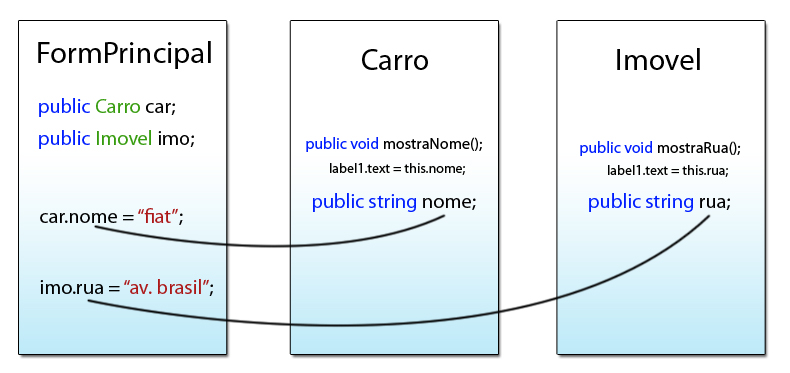
\includegraphics[width=\textwidth]{images/valoresForms.jpg}
            \caption{Ilustrando como � poss�vel o compartilhamento de valores entre forms}
        \end{center}
    \end{figure}
\end{frame}

\subsection{Posicionando e estado dos formul�rios na tela}

\begin{frame}
    \frametitle{Posicionando os formul�rios na tela \emph{StartPosition}}
    \begin{itemize}
        \item Est�tica do projeto;
        \item Propriedade \emph{StartPosition}:
        \begin{itemize}
            \item \emph{CenterScreen}: centro da tela;
            \item \emph{Manual}: Deve-se especificar manualmente os
            valores:
            \begin{itemize}
                \item Posicionamento ${x, y}$ do formul�rio na tela.
            \end{itemize}
        \end{itemize}
    \end{itemize}
\end{frame}

\begin{frame}
    \frametitle{Estado inicial do formul�rio}
    \begin{itemize}
        \item \emph{Normal}: Abre o formul�rio em seu estado inicial;
        \item \emph{Minimized}: Abre o formul�rio minimizado na barra de
        tarefas;
        \item \emph{Maximized}: Abre o formul�rio maximizado.
    \end{itemize}
\end{frame}

\subsection{Controlando os eventos dos formul�rios}

\begin{frame}
    \frametitle{Controlando os eventos dos formul�rios}
    \begin{itemize}
        \item A��es atribu�das ao comportamento do formul�rio;
        \item Ao ocorrer um evento, um bloco de c�digo � executado (\emph{Manipulador de Evento});
        \item Nomea��o padr�o combina o nome do objeto com o evento correspondente ligando-os por um
        underline:
        \begin{itemize}
            \item exemplo: button1\_Click; form1\_Load.
        \end{itemize}
    \end{itemize}
\end{frame}

\subsection{Aplica��es de exemplo}

\begin{frame}
    \frametitle{Aplica��es de exemplo}
    Para fixar o conte�do estudado, vamos analisar as seguintes
    aplica��es:
    \begin{itemize}
        \item Aplica��o com janelas MDI (MDIApplication);
        \item Aplica��o com formul�rios \textcolor[rgb]{0.00,0.50,0.00}{Verde} e \textcolor[rgb]{0.98,0.00,0.00}{Vermelho} (VerdeVermelho);
        \item Aplica��o com posicionamento das janelas (PosicaoForm);
        \item Aplica��o com eventos dos formul�rios (EventosForm);
        \item Aplica��o com intera��o de objetos entre formul�rios
        (InteracaoFormularios);
    \end{itemize}
\end{frame}

\subsection{Exerc�cios para praticar}

\begin{frame}
    \frametitle{Exerc�cios para praticar}
    \begin{enumerate}
        \item Em uma aplica��o MDI, implemente $n$ filhos para uma
        aplica��o, cada filho dessa aplica��o ser� um bloco de
        notas que dever� abrir e salvar arquivos de locais
        selecionados pelo usu�rio. O programa deve mostrar o n�mero
        do filho, e ordenar as janelas conforme a aplica��o MDI de
        exemplo.
        \item Fa�a uma aplica��o que altere atrav�s de um formul�rio
        principal a cor, o tamanho, o posicionamento e um label de
        um outro formul�rio no projeto.
        \item Utilizando o primeiro exerc�cio e os conceitos de eventos, implemente:
        \begin{itemize}
            \item Mensagem de boas vindas ao abrir o programa;
            \item Confirma��o quando o usu�rio tentar sair do
            programa;
        \end{itemize}
    \end{enumerate}
\end{frame}


\subsection{Exerc�cio para entregar}

\begin{frame}[t,allowframebreaks]
    \frametitle{Exerc�cio para entregar}
    Uma empresa solicitou a cria��o de um programa que vai registrar
    em um �nico arquivo texto seus clientes, clientes preferenciais
    e seus fornecedores.
    A estrutura para a cria��o do arquivo pode ser analisada no
    seguinte diagrama de classes:
    \begin{figure}[htb]
        \begin{center}
            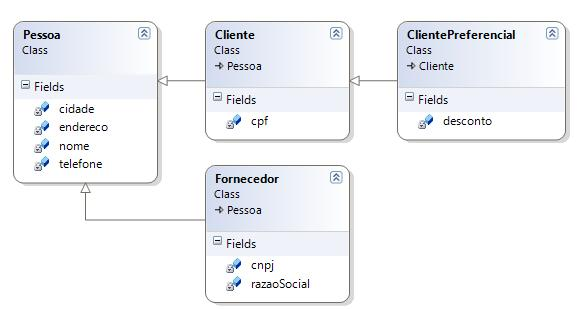
\includegraphics[width=8cm]{images/diagramaExWindowApp.jpg}
            \caption{Diagrama de classes a ser implementado}
        \end{center}
    \end{figure}
    Existe um projeto criado pelo analista de sistema dispon�vel
    para facilitar a implementa��o do projeto, esse arquivo se chama
    ExWindowApp.rar (dispon�vel no moodle);
    O arquivo de sa�da deve ser formatado da seguinte maneira:
    \texttt{\lstinputlisting[language=C, label=exWindowApp,
    caption={Arquivo texto utilizado pela empresa}]{cods/arquivoSaida.txt}}
    R:F:: indica que os pr�ximos registros ser�o fornecedores, --
    indica a separa��o entre registros, R:C:: indica o registro de
    clientes e R:CP :: indica o registro de clientes preferenciais.

    � importante que o programa seja feito em m�ltiplos formul�rios,
    um formul�rio para cadastro de fornecedores, outro para cadastro
    de clientes e outro para o cadastro de clientes preferenciais. O
    programa dever� trabalhar com listas de objetos. O programa
    deve ter ainda a op��o: salvar dados, a qual
    dever� localizar um local para gerar o arquivo texto conforme a
    formata��o solicitada.

    Esse projeto engloba a maioria das funcionalidades estudadas at�
    o momento e valer� 20 pontos na nota dos exerc�cios.

    Data da entrega: 17 de outubro.

    Dica: utilize os projetos j� montados e reaproveite seus
    c�digos.
\end{frame}

%\section{Conex�o com Banco de Dados}

\subsection{O que � o ADO.NET ?}

\begin{frame}
    \frametitle{O que � o ADO.NET ?}
    \begin{itemize}
        \item Tecnologia baseada no ADO (\emph{Active Data Objects});
        \item Criado para trabalhar com um ambiente desconectado;
        \item Camada de persist�ncia em XML.
    \end{itemize}
\end{frame}

\subsection{Os namespaces relacionados ao ADO.NET}

\begin{frame}
    \frametitle{Os namespaces relacionados ao ADO.NET}
    \begin{itemize}
        \item Os namespaces utilizados para trabalhar com ADO.NET:
        \begin{itemize}
            \item \emph{System.Data}: Infra-estrutura b�sica para trabalharmos com qualquer base de dados relacional;
            \item \emph{System.Data.Common}: Interfaces comuns a todos os bancos de dados;
            \item \emph{System.Data.SqlClient}: Biblioteca de acesso ao SQL Server;
            \item \emph{System.Data.OleDb}: Biblioteca de acesso para bancos de dados que suportam OleDb;
            \item \emph{System.Data.SqlTypes}: Defini��o dos tipos nativos do SQL Server;
            \item \emph{System.XML}: Cont�m as classes para manipula��o de documentos XML.
        \end{itemize}
    \end{itemize}
\end{frame}

\subsection{O modelo de execu��o do ADO.NET}

\begin{frame}[t,allowframebreaks]
    \frametitle{O modelo de execu��o do ADO.NET}
    \begin{itemize}
        \item M�ltiplas bases de dados simultaneamente;
        \item � poss�vel armazenar duas tabelas de diferentes bancos de dados;
        \item Estrutura respons�vel pelo armazenamento dos dados: \emph{DataSet};
        \item Os \emph{DataSet} cont�m um conjunto de objetos (\emph{DataTables}) que representam resultados tabulares extra�dos da base de dados.
    \end{itemize}

    \begin{figure}[htb]
        \begin{center}
            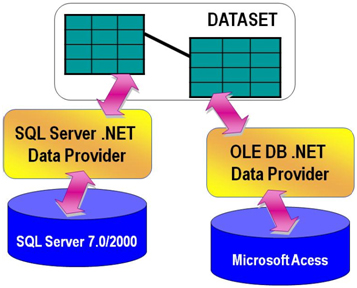
\includegraphics[width=6cm]{images/dataProvider.jpg}
            \caption{Esquema acesso ao banco de dados}
        \end{center}
    \end{figure}

    \begin{itemize}
        \item Para extrair os dados: .\emph{NET Data Providers};
        \item \emph{Data Providers}: bibliotecas de classes especializadas para o acesso a um tipo de banco de dados relacional;
        \item Por serem uma implementa��o espec�fica, s�o mais eficientes que bibliotecas gen�ricas como OLEDB ou ODBC;
        \item Apesar de cada implementa��o ser espec�fica para o banco de dados, possuem uma estrutura em comum.
    \end{itemize}
\end{frame}

\subsection{O modelo de execu��o em um ambiente conectado}

\begin{frame}
    \frametitle{O modelo de execu��o em um ambiente conectado}
    \begin{itemize}
        \item O ADO.NET � capaz de trabalhar com dois modelos, o modelo conectado e o modelo desconectado;
        \item No modelo conectado: necess�rio manter a conex�o aberta enquanto s�o realizadas as opera��es de leitura e grava��o;
        \item Para trabalharmos com o modelo conectado do ADO.NET devemos seguir a seguinte ordem:
        \begin{enumerate}
            \item \emph{XxxConnection}: utilizado para estabelecer a conex�o com o banco;
            \item \emph{XxxCommand}: � um objeto utilizado para enviar comandos a base de dados;
            \item \emph{XxxDataReader}: � um objeto utilizado para ler dados de um comando executado.
        \end{enumerate}
    \end{itemize}
\end{frame}

\subsection{O modelo de execu��o em um ambiente desconectado}

\begin{frame}[t,allowframebreaks]
    \frametitle{O modelo de execu��o em um ambiente desconectado}
    \begin{itemize}
        \item Utiliza outros objetos;
        \item \emph{DataSet}: armazena e manipula os dados em mem�ria;
        \item \emph{XxxDataAdapter}: extrai e envia as altera��es ao banco de dados;
        \item Os passos para extra��o e manipula��o dos dados em um ambiente desconectado s�o:
        \begin{enumerate}
            \item � aberta uma conex�o utilizando um objeto \emph{XxxConnection};
            \item � criado um objeto do tipo \emph{XxxDataAdapter}: dados para memoria $\rightarrow$ aramazena altera��es;
            \item m�todo \emph{Fill} do \emph{XxxDataAdapter} para extrair os dados da base e armazenar em um \emph{DataSet};
            \item Fechamos a conex�o com o banco pois os dados;
            \item � poss�vel inserir, remover ou alterar registros do \emph{DataSet};
            \item Ao finalizar as altera��es, restabelecemos a conex�o com o banco de dados para enviar as altera��es;
            \item Utilizase o comando \emph{XxxCommandBuilder} para gerar as strings sql que v�o alterar o \emph{XxxDataAdapter};
            \item Utilizando o m�todo \emph{Update} do \emph{DataAdapter}, enviamos as altera��es para o banco de dados;
            \item Ao finalizar o processo, fechamos a conex�o com o banco de dados.
        \end{enumerate}
    \end{itemize}
\end{frame}

\subsection{Estabelecendo uma conex�o com um banco de dados}

\begin{frame}
    \frametitle{Estabelecendo uma conex�o com um banco de dados}
    \begin{itemize}
        \item Primeiro passo para uma aplica��o que acessa dados de um banco;
        \item Cria-se uma inst�ncia (objeto) da classe que faz a conex�o com o banco;
        \item Ao criar essa inst�ncia informa-se uma \emph{Connection String} que cont�m par�metros para conex�o no banco, como usu�rio e senha;
        \item A \emph{string} de conex�o possui uma s�rie de par�metros que podem variar de acordo com o banco de dados utilizado;
        \item Os par�metros s�o separados por ponto e virgula.
    \end{itemize}
    \texttt{\texttt{\lstinputlisting[language=C, label=mdiFilha,
    caption={Padr�o para Connection Strings}]{cods/connectionStringDefault.txt}}}
\end{frame}

\begin{frame}
    \frametitle{Exemplos de Connection Strings}
    \texttt{\texttt{\lstinputlisting[language=C, label=mdiFilha,
    caption={Exemplos de Connection Strings}]{cods/connectionStringsGlobal.txt}}}
\end{frame}

\subsection{Criando comandos}

\begin{frame}[t,allowframebreaks]
    \frametitle{Criando comandos}
    \begin{itemize}
        \item � poss�vel executar comandos no banco atrav�s da classe: \emph{SqlCommand};
        \item Ao se criar uma inst�ncia deve-se informar a consulta SQL bem como a Conex�o com o banco;
        \item Esses par�metros podem ser informados no construtor ou atrav�s das propriedades \emph{CommandText} e \emph{Connection};
        \item Os SQL's informados podem ser de qualquer tipo:
        \begin{itemize}
            \item Retornando um conjunto de registros;
            \item Retornando um valor espec�fico;
            \item Sem retorno.
        \end{itemize}
        \item Para cada um desses casos existe um m�todo espec�fico para execu��o.
    \end{itemize}
    \texttt{\texttt{\lstinputlisting[language=C, label=mdiFilha,
    caption={Exemplo de utiliza��o do comando SqlCommand}]{cods/sqlCommand.txt}}}
\end{frame}

\subsection{Executando comandos}

\begin{frame}
    \frametitle{Executando comandos}
    \begin{itemize}
        \item Os m�todos de execu��o variam de acordo com a natureza do comando executado;
        \item Os tr�s m�todos mais comuns s�o:
        \begin{itemize}
            \item \emph{ExecuteNonQuery}: Para comandos que n�o executam consultas (querys);
            \item \emph{ExecuteScalar}: Para comandos que executam resultados escalares;
            \item \emph{ExecuteReader}: Para comandos que retornam conjuntos de dados.
        \end{itemize}
    \end{itemize}
\end{frame}

\subsubsection{O m�todo ExecuteNonQuery}

\begin{frame}
    \frametitle{O m�todo ExecuteNonQuery}
    \begin{block}{Defini��o}
        � utilizado quando queremos executar um comando que n�o retorna como
        resultado um conjunto de dados.
    \end{block}
    \begin{itemize}
        \item Utilizado para executar DCL (\emph{Data Control Language}) suportados pelo banco de dados;
        \item Opcionalmente podemos informar um par�metro para este m�todo para obter o n�mero de linhas afetadas pelo comando executado.
    \end{itemize}
    \texttt{\texttt{\lstinputlisting[language=C, label=mdiFilha,
    caption={Exemplo de utiliza��o do comando ExecuteNonQuery}]{cods/executeNonQuery.txt}}}
\end{frame}

\subsubsection{O m�todo ExecuteScalar}

\begin{frame}
    \frametitle{O m�todo ExecuteScalar}
    \begin{block}{Defini��o}
        � utilizado para comandos que retornam valores escalares, ou seja,
        valores �nicos.
    \end{block}
    \begin{itemize}
        \item Em geral � utilizado para comandos que retornam uma contagem de registros;
        \item Este comando pode retornar qualquer tipo de dado.
    \end{itemize}
    \texttt{\texttt{\lstinputlisting[language=C, label=mdiFilha,
    caption={Exemplo de utiliza��o do comando ExecuteScalar}]{cods/executeScalar.txt}}}
\end{frame}

\subsubsection{O m�todo ExecuteReader}

\begin{frame}[t,allowframebreaks]
    \frametitle{O m�todo ExecuteReader}
    \begin{block}{Defini��o}
        � utilizado para executar consultas (\emph{querys}) que retornam um conjunto de
        dados.
    \end{block}
    \begin{itemize}
        \item Este m�todo tem como resultado um objeto do tipo \emph{SqlDataReader}.
        \item A classe \emph{SqlDataReader} representa um cursor aberto no banco de dados com os dados retornados;
        \item Para lermos os dados de um \emph{DataReader}, � necess�rio executamos o m�todo \emph{Read};
        \item Com o \emph{DataReader} n�o � possivel executar nenhuma outra opera��o com a mesma conex�o aberta, por isso deve-se fechar ao t�rmino da execu��o.
    \end{itemize}
    \texttt{\texttt{\lstinputlisting[language=C, label=mdiFilha,
    caption={Exemplo de utiliza��o do comando ExecuteReader}]{cods/executeReader.txt}}}
\end{frame}

\subsection{Passando par�metros}

\begin{frame}[t,allowframebreaks]
    \frametitle{Passando par�metros}
    \begin{itemize}
        \item � poss�vel passar par�metros para os objetos da classe \emph{SqlCommand};
        \item Para indicarmos par�metros nas \emph{querys} utilizamos o s�mbolo @ como prefixo para indicar um par�metro;
        \item Esta sintaxe pode variar de acordo com o banco de dados utilizado (o Oracle utiliza ":" por exemplo);
        \item Depois de indicar os par�metros na query, � preciso adicionar objetos do tipo \emph{SqlParameter} na cole��o de par�metros do \emph{SqlCommand}.
    \end{itemize}
    \texttt{\texttt{\lstinputlisting[language=C, label=mdiFilha,
    caption={Exemplo de utiliza��o de par�metros}]{cods/parametros.txt}}}
\end{frame}

\subsection{O que � um DataSet?}

\begin{frame}
    \frametitle{O que � um DataSet?}
    \begin{block}{Defini��o}
        O \emph{DataSet} � uma classe capaz de armazenar m�ltiplos
        resultados tabulares em uma mesma estrutura.
    \end{block}
    \begin{itemize}
        \item Composto por \emph{DataTables} que representam estes resultados tabulares;
        \item Para extrairmos dados da base de dados e preenchermos o \emph{DataSet} utilizamos a classe \emph{DataAdapter};
    \end{itemize}
\end{frame}

\subsection{O que � um DataAdapter?}

\begin{frame}
    \frametitle{O que � um DataAdapter?}
    \begin{block}{Defini��o}
        O \emph{DataAdapter} � a classe respons�vel por fazer a intera��o
        entre a base de dados e o \emph{DataSet}.
    \end{block}
    \begin{itemize}
        \item Capaz de executar os quatro comandos b�sicos de um banco de dados (\emph{Insert, Update, Delete, Select});
        \item Para extrairmos dados da base de dados e preenchermos o \emph{DataSet} utilizamos a classe \emph{DataAdapter};
    \end{itemize}
\end{frame}

\subsection{Criando um DataSet e um DataAdapter}

\begin{frame}
    \frametitle{Criando um DataSet e um DataAdapter}
    \begin{block}{Instru��es}
        Quando criamos um \emph{DataAdapter} � poss�vel informar uma
        \emph{query} e uma conex�o para a extra��o dos dados.
    \end{block}
    \texttt{\texttt{\lstinputlisting[language=C, label=mdiFilha,
    caption={Criando um DataSet e um DataAdapter}]{cods/dataAdapterDataSet.txt}}}
\end{frame}

\subsection{Criando e preenchendo um DataSet}

\begin{frame}
    \frametitle{Criando e preenchendo um DataSet}
    \begin{block}{Instru��es}
        Para criar um novo \emph{DataSet} basta utilizar o comando New e
        criar um novo objeto. Para preencher um \emph{dataset} utilizando um
        \emph{DataAdapter}, devemos utilizar o m�todo \emph{Fill} do
        \emph{DataAdapter}, informando o \emph{DataSet} e nome da tabela a
        ser criada no \emph{DataSet}.
    \end{block}
    \texttt{\texttt{\lstinputlisting[language=C, label=mdiFilha,
    caption={Criando e preenchendo um DataSet}]{cods/preenchendoDataSet.txt}}}
\end{frame}

\section{Apresenta��o do Projeto Integrador}

\subsection{Etapas para apresenta��o do projeto integrador}

\begin{frame}
    \frametitle{Etapas para apresenta��o do projeto integrador}
    \begin{itemize}
        \item Introdu��o;
        \item Metodologia;
        \item Tecnologia utilizada;
        \item O Sistema;
        \item Considera��es finais.
    \end{itemize}
\end{frame}

\subsubsection{Introdu��o}
\begin{frame}
    \frametitle{Introdu��o}
    \begin{itemize}
        \item O que �?
        \begin{itemize}
            \item Pequena descri��o em t�picos do sistema.
        \end{itemize}
        \item Quem auxiliar�?
        \begin{itemize}
            \item Pequena descri��o em t�picos de quem o sistema
            auxiliar� (atores).
        \end{itemize}
        \item A empresa?
        \begin{itemize}
            \item Descri��o da empresa para qual ser� desenvolvido o
            sistema.
        \end{itemize}
        \item Por que informatizar?
        \begin{itemize}
            \item Justificativa da necessidade do sistema
            desenvolvido no �mbito empresarial.
        \end{itemize}
    \end{itemize}
\end{frame}

\subsubsection{Metodologia}
\begin{frame}
    \frametitle{Metodologia}
    \begin{itemize}
        \item Qual a metodologia de desenvolvimento utilizada no processo?
        \begin{itemize}
            \item Pequena descri��o em t�picos da metodologia.
        \end{itemize}
        \item Artefatos gerados:
        \begin{itemize}
            \item Descri��o dos principais artefatos gerados.
        \end{itemize}
    \end{itemize}
\end{frame}

\subsubsection{Tecnologia utilizada}
\begin{frame}
    \frametitle{Tecnologia utilizada}
    \begin{itemize}
        \item Linguagem de programa��o:
        \begin{itemize}
            \item Descrever as funcionalidades aplicadas ao sistema dispon�veis pela linguagem de
            programa��o.
        \end{itemize}
        \item Persist�ncia de dados:
        \begin{itemize}
            \item Descrever as funcionalidades do SGBD utilizado
            para desenvolvimento do projeto.
        \end{itemize}
    \end{itemize}
\end{frame}

\subsubsection{O sistema}
\begin{frame}
    \frametitle{O sistema}
    \begin{itemize}
        \item Objetivos do sistema;
        \item Levantamento de requisitos:
        \begin{itemize}
            \item Qual a base para o desenvolvimento do projeto?
        \end{itemize}
        \item Pontos fortes:
        \begin{itemize}
            \item Descrever os pontos fortes do sistema desenvolvido
            (qual a contribui��o para a empresa?).
        \end{itemize}
        \item Pontos fracos:
        \begin{itemize}
            \item Descrever os pontos fracos do sistema desenvolvido
            (que mudan�as ou complica��es o sistema pode gerar?).
        \end{itemize}
        \item Facilidades encontradas no desenvolvimento do sistema;
        \item Dificuldades encontradas no desenvolvimento do
        sistema;
        \item Prot�tipos de tela gerados.
    \end{itemize}
\end{frame}


\end{document}
